\section{Приложение ТЕСТ}

\subsection{Условие задания}

Создать приложение для проведения тестирования.

Должно содержать:
\begin{enumerate}
    \item Набор вопросов по какой-то теме (и вопросы и ответы должны быть реальные) -не менее 10
    \item Вопросы должны выбираться случайным образом.
    \item Вопросы должны быть нескольких типов - "Да/нет", Выбор одного ответа, Выбор нескольких ответов, Короткий ответ.
    \item Необходимо создать сообщения для правильного и неправильного ответа (Молодец, Не правильно и т.д.)
    \item Необходимо подсчитать количество правильных ответов и вывести результат.
\end{enumerate}

\subsection{Вид формы в конструкторе}


Создано две формы приложения, содержащие три элемента TextBox, три элемента Label, один элемент Button, один элемент ErrorProvider для обработки ошибок и один элемент groupBox с четыремя элементами checkbox. Вид окна вопроса представлен на рисунке \ref{task9_form1} \cite{зиборов2011ms}.
\begin{figure}[H]
    \centering
    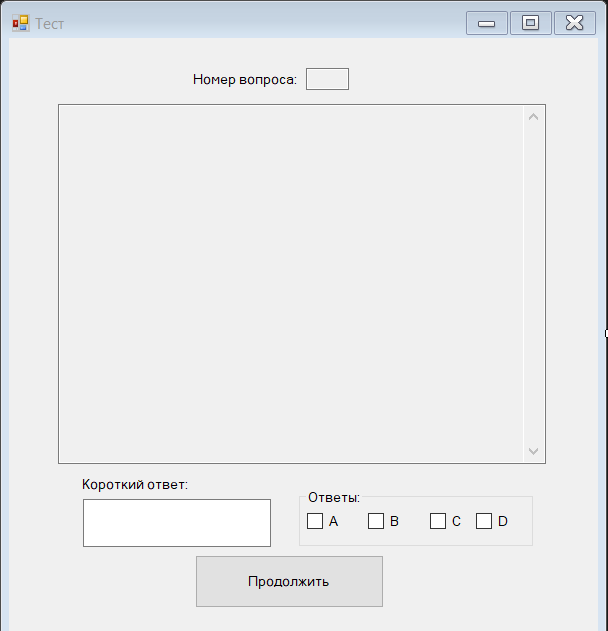
\includegraphics[width=0.8\linewidth]{lections/img/task9_form1.png}
    \caption{Окно вопросов приложения «Тест» открытое в конструкторе}
    \label{task9_form1}
\end{figure}

Вид окна результата представлен на рисунке \ref{task9_form2}.
\begin{figure}[H]
    \centering
    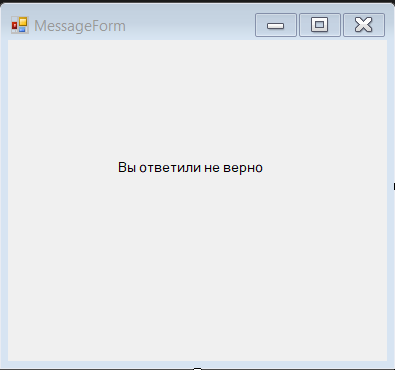
\includegraphics[width=0.5\linewidth]{lections/img/task9_form2.png}
    \caption{Окно результата приложения «Тест» открытое в конструкторе}
    \label{task9_form2}
\end{figure}


\subsection{Таблица с описанием переименованных элементов формы}
Все измененные элементы формы указаны в таблице \ref{task9_attributes}.

\begin{longtable}{|l|l|l|}
\caption{Значения атрибутов элементов в приложении <<Тест>>}\label{task9_attributes}\\
\hline
\textbf{\begin{tabular}[c]{@{}l@{}}Описание элементов\\ формы\end{tabular}}           & \textbf{\begin{tabular}[c]{@{}l@{}}Список измененных\\ атрибутов\end{tabular}} & \textbf{\begin{tabular}[c]{@{}l@{}}Новое значение\\ атрибута\end{tabular}} \\ \hline
\endfirsthead
%
\endhead
%
Форма MyForm                                                                          & Text                                                                           & Тест                                                                       \\ \hline
\multirow{2}{*}{TextBox номера вопроса}                                               & Name                                                                           & countBox                                                                   \\ \cline{2-3} 
                                                                                      & ReadOnly                                                                       & True                                                                       \\ \hline
\multirow{2}{*}{TextBox короткого ответа}                                             & Name                                                                           & shortAns                                                                   \\ \cline{2-3} 
                                                                                      & Multiline                                                                      & True                                                                       \\ \hline
\multirow{3}{*}{TextBox текста вопроса}                                               & Name                                                                           & questBox                                                                   \\ \cline{2-3} 
                                                                                      & Multiline                                                                      & True                                                                       \\ \cline{2-3} 
                                                                                      & ReadOnly                                                                       & True                                                                       \\ \hline
\multirow{2}{*}{Кнопка ответа}                                                        & Name                                                                           & act                                                                        \\ \cline{2-3} 
                                                                                      & Text                                                                           & Продолжить                                                                 \\ \hline
\multirow{2}{*}{\begin{tabular}[c]{@{}l@{}}GroupBox вариантов\\ ответа\end{tabular}}  & Name                                                                           & answerGroup                                                                \\ \cline{2-3} 
                                                                                      & Text                                                                           & Ответы:                                                                    \\ \hline
\multirow{2}{*}{\begin{tabular}[c]{@{}l@{}}CheckBox варианта ответа\\ А\end{tabular}} & Name                                                                           & answerA                                                                    \\ \cline{2-3} 
                                                                                      & Text                                                                           & A                                                                          \\ \hline
\multirow{2}{*}{\begin{tabular}[c]{@{}l@{}}CheckBox варианта ответа\\ B\end{tabular}} & Name                                                                           & answerB                                                                    \\ \cline{2-3} 
                                                                                      & Text                                                                           & B                                                                          \\ \hline
\multirow{2}{*}{\begin{tabular}[c]{@{}l@{}}CheckBox варианта ответа\\ C\end{tabular}} & Name                                                                           & answerC                                                                    \\ \cline{2-3} 
                                                                                      & Text                                                                           & C                                                                          \\ \hline
\multirow{2}{*}{\begin{tabular}[c]{@{}l@{}}CheckBox варианта ответа\\ D\end{tabular}} & Name                                                                           & answerD                                                                    \\ \cline{2-3} 
                                                                                      & Text                                                                           & D                                                                          \\ \hline

\end{longtable}


\subsection{Примеры правильной и неправильной работы}
После запуска программы на экране появляется окно на рисунке \ref{task9_launch1}.
\begin{figure}[H]
    \centering
    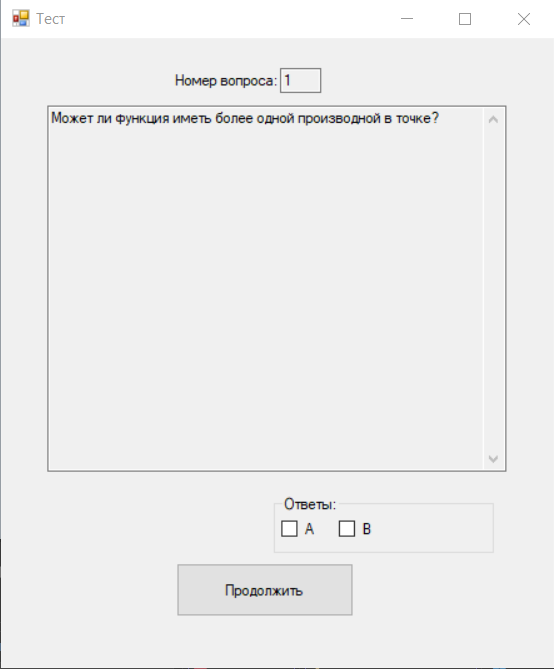
\includegraphics[width=0.8\linewidth]{lections/img/task9_launch1.png}
    \caption{Запуск программы}
    \label{task9_launch1}
\end{figure}

После выбора варианта ответа и нажатия кнопки "Продолжить" ( на рисунке \ref{task9_launch2}).

\begin{figure}[H]
    \centering
    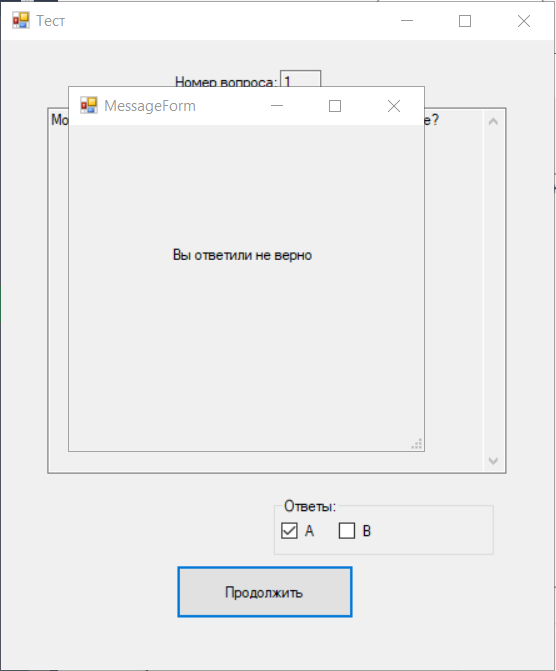
\includegraphics[width=0.8\linewidth]{lections/img/task9_launch2.png}
    \caption{Отфильтрованная таблица}
    \label{task9_launch2}
\end{figure}

При выбрать одновременно "Да" и "Нет" вылазит ошибка (на рисунке \ref{task9_launch3})
\begin{figure}[H]
    \centering
    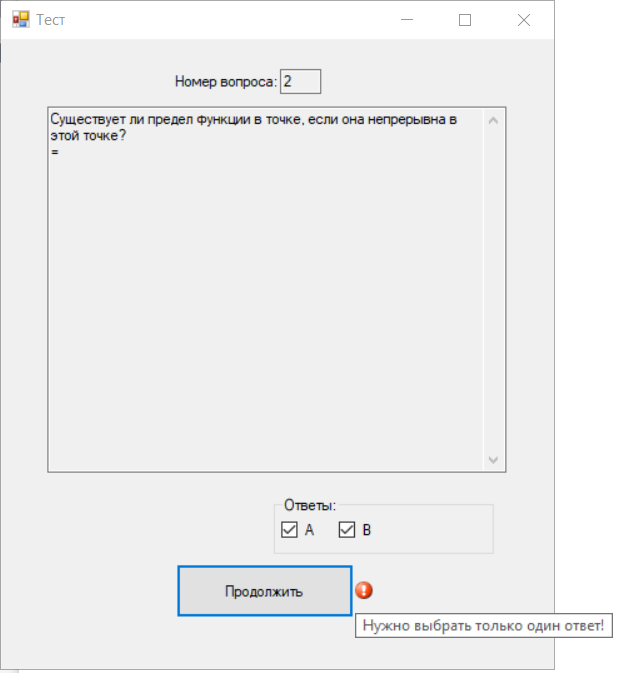
\includegraphics[width=0.8\linewidth]{lections/img/task9_launch3.png}
    \caption{Ошибка формата ввода}
    \label{task9_launch3}
\end{figure}

\subsection{Примеры исходного кода}


Функция считывания вопроса из вектора.
\begin{minted}[style=bw,
 linenos=true,
 breaklines=true,
 numbersep=5pt,
 tabsize=2,
 fontsize=\small,
 bgcolor=white]{cpp}
std::string ReadAnswer() {
	int i = RandIndex->at(iter);
	Quest temp = Questions->at(i);
	if (temp.getType() == "ДаНет") {
		return YesNoRead();
	}
	else if (temp.getType() == "ОдинОтвет") {
		return OneAnswerRead();
	}
	else if (temp.getType() == "НесколькоОтветов") {
		return SomeAnswersRead();
	}
	else {
		return ShortAnswerRead();
	}

}
\end{minted}
Другие фрагменты кода расположены в приложении \ref{app:test}.
\sectionbreak